\documentclass[a4paper,14pt]{extarticle} %размер бумаги устанавливаем А4, шрифт 14пунктов
\usepackage[T2A]{fontenc}
\usepackage[utf8]{inputenc}%включаем свою кодировку: koi8-r или utf8 в UNIX, cp1251 в Windows
\usepackage[english,russian]{babel}%используем русский и английский языки с переносами
\usepackage{amssymb,amsfonts,amsmath,mathtext,cite,enumerate,float} %подключаем нужные пакеты расширений

\usepackage{alltt}
\usepackage{fancyvrb}
%шрифт Times New Roman
%\usepackage{fontspec}
%\setmainfont{Times New Roman}
%\setallmainfonts{Times New Roman}

\usepackage{titlesec}
\usepackage{xcolor}
\usepackage{hyperref}
\usepackage{graphicx}
\graphicspath{{pictures/}}

\makeatletter
\renewcommand{\@biblabel}[1]{#1.} % Заменяем библиографию с квадратных скобок на точку:
\makeatother

\usepackage{geometry} % Меняем поля страницы
\geometry{left=3cm}% левое поле
\geometry{right=15mm}% правое поле
\geometry{top=2cm}% верхнее поле
\geometry{bottom=2cm}% нижнее поле
\linespread{1.5}

\usepackage{indentfirst} % отделять первую строку раздела абзацным отступом
\setlength\parindent{5ex}
\usepackage{tikz}
\usepackage{pgfplots}
%links
\usepackage{url}

\usepackage[tableposition=top,singlelinecheck=false, justification=centering]{caption}
\usepackage{subcaption}

% маркированные списки
\renewcommand{\labelitemi}{--}
\renewcommand{\labelitemii}{--}
% нумерованные списки
\renewcommand{\labelenumi}{\asbuk{enumi})}
\renewcommand{\labelenumii}{\arabic{enumii})}

% номер сноски со скобкой
\renewcommand*{\thefootnote}{\arabic{footnote})}
\renewcommand{\footnoterule}{%
\kern -3pt
\hrule width 40mm height .4pt
\kern 2.6pt
}

%иллюстрации и таблицы
\DeclareCaptionLabelFormat{gostfigure}{Рисунок #2}
\DeclareCaptionLabelFormat{gosttable}{Таблица #2}
\DeclareCaptionLabelSeparator{gost}{~---~}
\captionsetup{labelsep=gost}
\captionsetup*[figure]{labelformat=gostfigure}
\captionsetup*[table]{labelformat=gosttable}
\renewcommand{\thesubfigure}{\asbuk{subfigure}}

\usepackage{tocloft}
\renewcommand{\cftsecleader}{\cftdotfill{\cftdotsep}}
%\renewcommand{\cfttoctitlefont}{\Large\filcenter}
%\setcounter{page}{3} %нумерация страниц с 3

\usepackage{listings}
\lstset{
frame=single,
breaklines=true
}
\author{Глушенкова А. Ю.}
\title{Морской бой}
\begin{document}
\begin{titlepage}
\begin{center}

ГУАП\\
КАФЕДРА № 51\\
\vspace{2cm}

\begin{flushleft}
ПРЕПОДАВАТЕЛЬ
\begin{tabular}{|l|l|l|}
\hline
доц., канд. техн. наук & & Е.М. Линский\\
\hline
должность, уч. степень, звание & подпись, дата & инициалы, фамилия\\
\hline
\end{tabular}
\end{flushleft}

\vspace{3cm}

{\Large ОТЧЕТ О КУРСОВОЙ РАБОТЕ\\}
\vspace{0.3cm}
{\Large СЕТЕВАЯ ИГРА КРЕСТИКИ-НОЛИКИ}

\vspace{0.7cm}

\begin{center}
по курсу: ТЕХНОЛОГИИ ПРОГРАММИРОВАНИЯ
\end{center}

\vspace{4cm}

\begin{flushleft}
РАБОТУ ВЫПОЛНИЛА
\begin{tabular}{|l|l|l|}
\hline
СТУДЕНТКА ГР. № 5723 & & Глушенкова А. Ю.\\
\hline
& подпись, дата & инициалы, фамилия\\
\hline
\end{tabular}
\end{flushleft}

\vspace{2cm}

Санкт-Петербург 2020

\end{center}
\end{titlepage}
\renewcommand{\chaptername}{Раздел}
\renewcommand{\figurename}{Рисунок}

\newpage
\setcounter{page}{2}
\section*{Оглавление}
\large
\begin{itemize}
\item{Функциональная спецификация.............................................3}
\item{Руководство пользователя......................................................4}
\item{Oписание архитектуры игры.................................................12}
\item{Oписание наиболее важных классов.....................................14}
\item{Тестирование.........................................................................17}
\end{itemize}

\newpage
\section*{Фукнциональная спецификация}
\paragraph{\largeБазовая версия\\}
\normalsize
Сетевая игра крестики-нолики будет две реализации: серверную и клиентскую, которые обе используют TCP соединение. Клиент будет подключаться к серверу с определенным ip. Игра имеет графический интерфейс.\\ 
Клиенту при заходе на сервер будет предложена аутентификация или регистрация, если у него нет аккаунта. Каждый игрок должен иметь уникальный логин.\\
Игрок может либо создать новую доску, либо присоединиться к уже созданной. Игра ведется, пока у одного из игрока не будет 5 одинаковых символов в ряд или по диагонали. Для каждого игрока ведется подсчет очков: 3 - победа, 2 - ничья, 1 - проигрыш. После окончания игры, игроку будет предложено начать еще одну или выйти. 


\vspace{1cm}
\paragraph{\large\\}
\normalsize


\newpage
\section*{Руководство пользователя}
\largeДанная программа делится на 2 части: клиент и сервер. Чтобы программа работала полностью, вы должны сначала запустить файл Server с помощью Maven в командной строке. 
\begin{figure}[h]
\centering
\includegraphics[width=1\linewidth]{MAVENSERVER.jpg}
\caption{Запуск сервера}
\label{fig:mpr}
\end{figure}

После этого в отдельной  командной  строке  запустите  файл клиента с помощью Maven.
\begin{figure}[h]
	\centering
	\includegraphics[width=1\linewidth]{MAVENCLIENT.jpg}
	\caption{Запуск клиента}
	\label{fig:mpr}
\end{figure}

\newpage

После запуска  программы игрока (клиента), на экран будет выведен вопрос, имеет ли клиент учетную запись на сервере в следующей форме:

\begin{figure}[h]
	\centering
	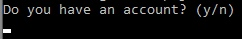
\includegraphics[width=0.5\linewidth]{ENTER.jpg}
	\caption{Вход пользователя}
	\label{fig:mpr}
\end{figure}
Необходимо ответить на вопрос y(yes) или n(no). При вводе иных символов, будет также выводится это сообщение.
\begin{figure}[h]
	\centering
	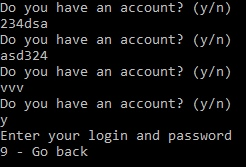
\includegraphics[width=0.5\linewidth]{ENTER4.jpg}
	\caption{Вход пользователя (вариации ответов)}
	\label{fig:mpr}
\end{figure}
\newpage
При вводе y пользователю необходимо ввести данные своей учетной записи. Если же он ошибся, то он может вернуться обратно и зарегистрироваться. Все учетные записи хранятся на сервере.
\begin{figure}[h]
	\centering
	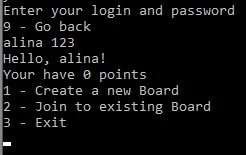
\includegraphics[width=0.5\linewidth]{ENTER5.jpg}
	\caption{Вход пользователя (вариации ответов)}
	\label{fig:mpr}
\end{figure}

При отсутствии учетной записи, клиент может зарегистрироваться: 
\begin{figure}[h]
	\centering
	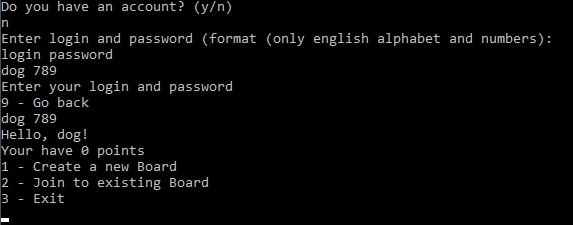
\includegraphics[width=0.7\linewidth]{REG6.jpg}
	\caption{Регистрация}
	\label{fig:mpr}
\end{figure}

\newpage
Зайдя в учетную запись, клиент увидит перед собой меню следующего вида:
\begin{figure}[h]
	\centering
	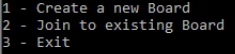
\includegraphics[width=0.8\linewidth]{MENU7.jpg}
	\caption{Главное меню}
	\label{fig:mpr}
\end{figure}

Если нажать 1, то вы создадите новую доску и будете ожидать подключение другого игрока. При этом вы будете играть крестиком. Вы ходите первым.
Если нажать 2, то вы присоединитесь к уже существующей созданой доске и будуте играть ноликом. Вы ходите вторым.
После выбора действия, первый игрок должен ввести ход, а второй игрок ждет окончания хода первого игрока.
\begin{figure}[h]
\centering
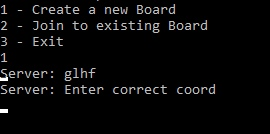
\includegraphics[width=0.8\linewidth]{MOVEX8.jpg}
\caption{Первый игрок}
\label{fig:mpr}
\end{figure}
\newpage
\begin{figure}[h]
	\centering
	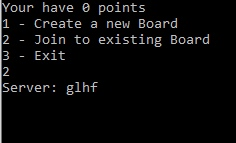
\includegraphics[width=0.8\linewidth]{MOVEO9.jpg}
	\caption{Второй игрок}
	\label{fig:mpr}
\end{figure}

\newpage
Необходимо ввести координаты в формате x y:
\begin{figure}[h]
\centering
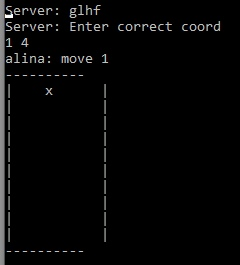
\includegraphics[width=0.4\linewidth]{MOVEXC10.jpg}
\caption{Ход первого игрока}
\label{fig:mpr}
\end{figure}

Второй игрок также получает отрисовку доски и просьбу ввести координаты:
\begin{figure}[h]
	\centering
	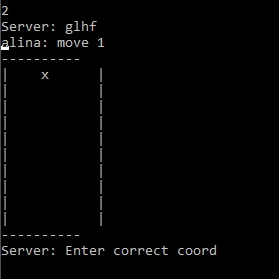
\includegraphics[width=0.4\linewidth]{SECOND11.jpg}
	\caption{Второй игрок}
	\label{fig:mpr}
\end{figure}

\newpage
После хода второго игрока:
\begin{figure}[h]
	\centering
	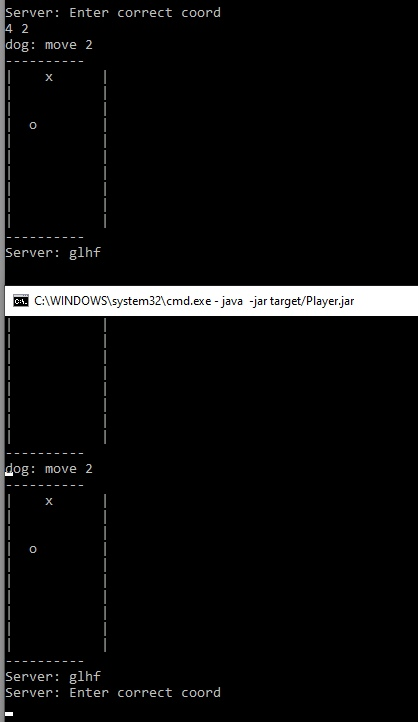
\includegraphics[width=0.5\linewidth]{MOVES12.jpg}
	\caption{Отображение досок}
	\label{fig:mpr}
\end{figure}

\newpage
\section*{Описание архитектуры игры}
\largeДанная игра состоит из четырех блоков:
\begin{itemize}
\item{Model.}
\item{View.}
\item{Client.}
\item{Server.}
\end{itemize}
\qquad
Взаимодействие блоков между собой.
Первым запускается Server. После, к нему подключаются Clients (Players). У каждого Client есть свои Model и View. Model отвечает за логику игры (сделать ход, определить закончилась игра или продолжаем играть дальше и т.д.), а View отвечает за отображение игры (вывод доски на экран, меню и общение с пользователем).

Между собой данные блоки взаимодейсвтуют так:
\newpage
\begin{figure}[h]
\centering
\includegraphics[width=0.8\linewidth]{Struct.jpg}
\caption{Архитектуры игры}
\label{fig:mpr}
\end{figure}

\newpage
\section*{Oписание наиболее важных классов}
\largeНаиболее важные классы данной игры это:
\begin{itemize}
\item{Model.}
\item{View.}
\item{Client.}
\item{Server.}
\end{itemize}
Назначение класса Model заключается в управление логикой игры. Данный класс отвечает за постановку хода (соответсвует введеный ход условиям или нет), определение конца игры и ее продолжения. Основные методы move, checkWinner.

Метод move делает ход, внутри проверяется правильность ввода. Метод checkWinner проверяет победителя, а следовательно проверяет конец игры.  

Класс View отвечает за вывод доски на экран и за вывод главного игрового меню. Основные методы данного класса это: printBoard, menu, login. 

Метод printBoard отвечат за вывод игрового поля на экран пользователя.

Методы menu, login отвечают за вывод меню и регистрацию.

Класс Client отвчетает за взаимодействие с пользователям. Он вызывает все меню, обрабатывает выбор пользователя в этих меню и осуществляет общение с сервером. Основными методами данного класса являются: createBoard, joinBoard.
 
Метод createBoard создает доску. Метод joinBoard присоединяется к доске.

Класс Server состоит из подкласса ClientTread, который общается с клиентом. Также есть подкласс AcceptThread, который ловит присоединяемых клиентов.

\newpage
\section*{Тестирование}
Тестирующим классом является класс ModelTest. Он тестирует публичные методы класса Model. Данный класс содержит следующие методы: 
\begin{itemize}
	\item{checkMoveTrue - даннный метод проверяет правильность работы метода move, который возвращает true, если ход был поставлен успешно, и возвращает false, если координаты выходят за поля или уже стоит ход другого игрока. Тестирующий метод подаёт на вход тестируемого метода некоторые входные данные и сравнивает результат с true.}
	\item{checkWinnerTrue - даннный метод проверяет правильность работы метода checkWinner, который возвращает некоторую константу, соответствующую победителю (1- первый, 2- второй). Тестирующий метод подаёт на вход тестируемого метода некоторые входные данные и сравнивает результат с константой, которая ожидается.}
\end{itemize}

\end{document}